% Brief overview of the observables that are measured
The observables we measured in the $1 + 1$D CDT model are the \emph{standard deviation} of the length profile $\sigma_\ell$ and the \emph{length covariance} $\rho_\ell(t)$ as introduced in section \ref{sec:observables}.
In this section we will present and discuss the results found for these observables.

\subsection{Pre-analysis}
% Determination of the equilibration time and correlation time
Before the actual measurements can be performed some data analysis need to be done beforehand.

\paragraph{Equilibration}
To be able to take measurements of the wanted observables in the Markov-chain Monte Carlo simulation the system needs to be thermalised. Which is to say that the system should be in a `typical' state, such that the expectation value of an observable at any timestep in the simulation is the same as any other.
We start the system in a non-typical, flat spacetime, so it takes some Markov-chain steps before the system is in equilibrium.
We want to only start measurements after this \emph{equilibration time}, so we need to estimate it to know when to start measuring.

Preferably one used the observable of interest to determine the equilibration time, however it is very difficult to quantify when a function like $\rho_\ell(t)$ has thermalised. So we determine the equilibration time using $\sigma_\ell$.
To determine when the system has equilibrated in terms of $\sigma_\ell$ we fit a function which converges exponentially towards the average value:
$\sigma(t) = \hat\sigma \qty(1 - e^{t/t_\text{eq}})$, where $t$ here is the Monte Carlo simulation time.
This works well because the initial state is flat thus having $\sigma_\ell = 0$, which over time goes towards some mean value and fluctuates around it.
This fitting procedure is visualised in Fig. \ref{fig:thermalisation}.
\begin{figure}[ht]
    \centering
    \begin{minipage}[t]{0.47\linewidth}
        \centering
        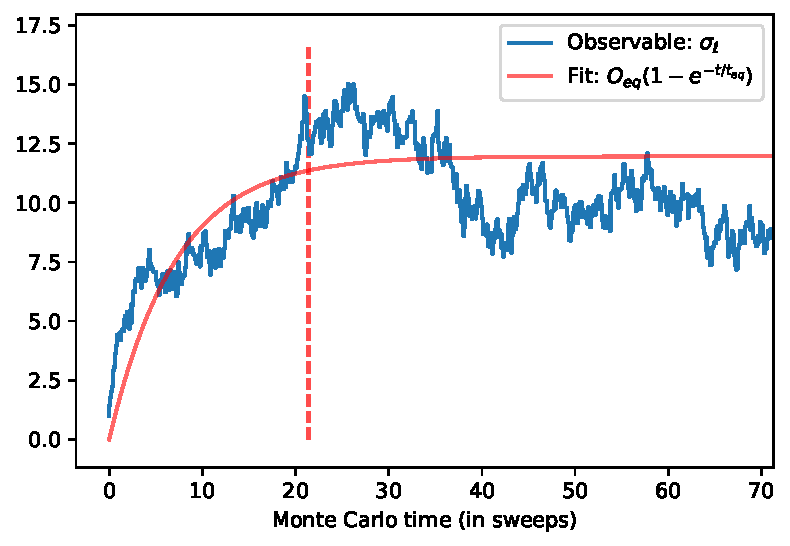
\includegraphics[width=0.95\linewidth]{img/teq_thermalisation.pdf}
        \caption{Visualisation of determination of thermalisation by fitting an exponential convergence. \textit{Marking at $3t_\text{eq}$}}
        \label{fig:thermalisation}
    \end{minipage}
    \hfill
    \begin{minipage}[t]{0.48\linewidth}
        \centering
        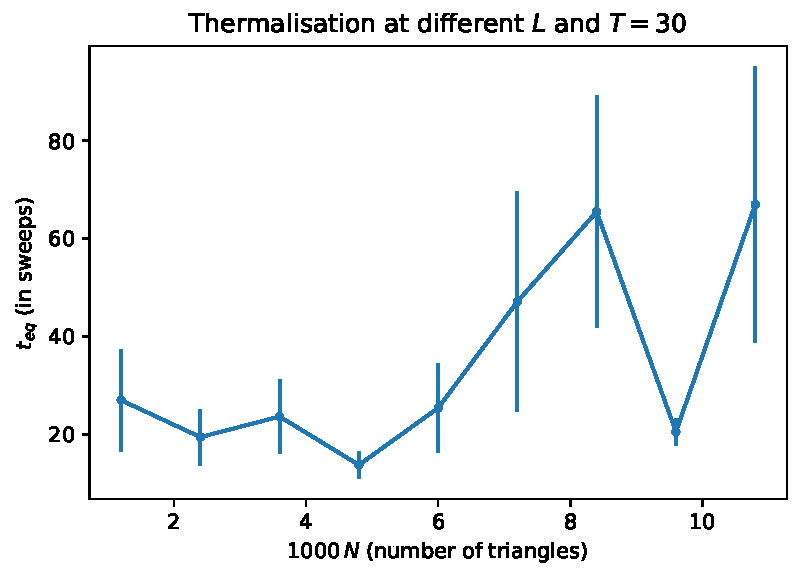
\includegraphics[width=0.95\linewidth]{img/teq-Ldep.pdf}
        \caption{Equilibration time for different sizes of $L$, based on 10 samples for each system size. Determined at move ratio $r=0.4$.}
        \label{fig:teq_Ldep}
    \end{minipage}
\end{figure}

So using this method we can estimate the equilibration time given a trace of $\sigma_\ell$.
Then instead of determining the equilibration time for every system we wish to measure, we attempted to determine the dependence of the equilibration time on different system sizes.
To do this we measured $t_\text{eq}$ for different values of $L$, and to obtain more accurate results and rough estimation of the error the measurements are repeated 10 times for each $L$.
This yields the results presented in Fig. \ref{fig:teq_Ldep} (note that $N = 2 L T$).

The found results show no clear dependence of $t_\text{eq}$ on the system size, and since we only wish to obtain an order estimate of it seems reasonable to assume that \emph{in terms of sweeps} the equilibration time is independent of the system size.
We then take the equilibration time to be $t_\text{eq} = 200 \, \text{sweeps}$ for all simulations to be safe.
This is a very cruse approximation of the equilibration time, but since $200 \,\text{sweeps}$ is not very much it seems unnecessary to put more work in a better estimate of the equilibration time.
%TODO%
% Maybe include the discussion of missing dependence on T for equilibration time?

\paragraph{Autocorrelation}
Once the system has thermalised, we can start to take measurements of the observables of interest.
However, after a single simulation timestep the newly obtained system is still very similar to the previous system, thus observables measured on these systems are by no means independent; they are in fact highly correlated.
Having many correlated measurements is not useful as they do not make the final estimate better, and take up a lot of unnecessary space and computation time.
Moreover, to be able to make and estimate of the error in the final results, it is crucial to know the correlation between measurements.

To estimate the correlation time we will again use the standard deviation as a value is much easier to work with than a function like the covariance.
The correlation time is then estimated the usual way by determining the autocorrelation of the standard deviation observable over for time:
\begin{equation*}
    \rho(t) = \frac{1}{Z} \, \sum_{i = 1}^{M - t} \qty(\sigma_{\ell, i} - \bar{\sigma}_\ell) \qty(\sigma_{\ell, i + t} - \bar{\sigma}_\ell),
\end{equation*}
where $\sigma_{\ell, i}$ is the $i$th measurement in a set of $M$ measurements of the standard deviation of the length profile, $\bar \sigma_\ell$ is the average standard deviation, and $Z$ is a normalisation factor such that $\rho(0) = 1$.

Now for long enough measurements we expect that the autocorrelation follows exponential decay with which we can define the correlation time $t_\text{cor}$ such that $\rho(t) \approx \exp(- t / t_\text{cor})$.
So to estimate $t_\text{cor}$ we simulate a long trace of $\sigma_\ell$ and fit an exponential decay to the autocorrelation of that trace.
To estimate the error on the estimate of the correlation time we can repeat the measurements several times; or to save on equilibration time we can simulate a very long trace and divide the trace up in batches which we treat as separate measurements.

We would like the autocorrelation to be as small as possible.
So now we have a method of determining the autocorrelation, we can use it to tune the move-ratio $r$ such that the autocorrelation is minimized.
To do this we estimate the autocorrelation for different move ratio's, the results of which are displayed in Fig. \ref{fig:tcor_rdep}.
\begin{figure}[ht]
    \centering
    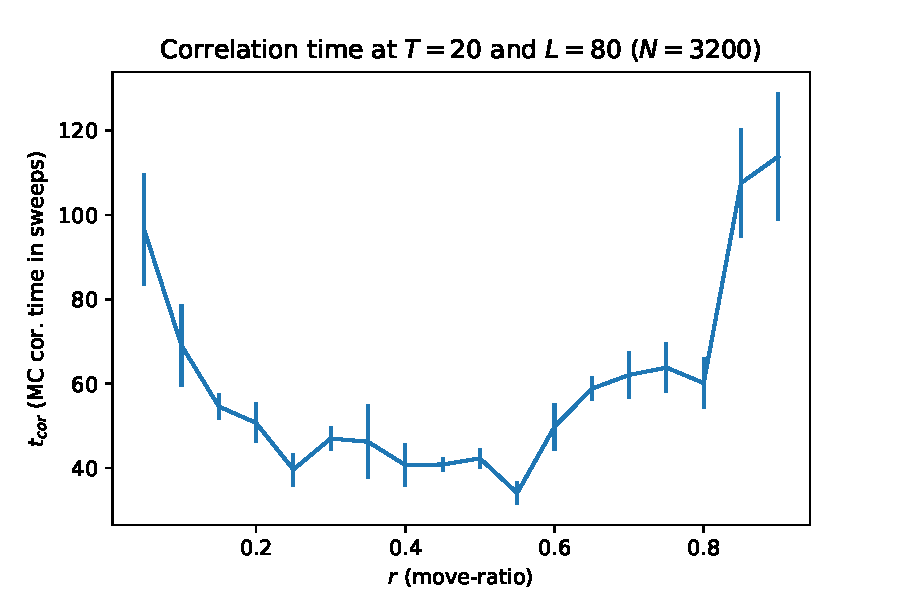
\includegraphics[width=0.7\linewidth]{img/tcor_r_t20_l80.pdf}
    \caption{Correlation time as function of the move-ratio.}
    \label{fig:tcor_rdep}
\end{figure}
From this figure one can clearly see that move ratio's close to $0$ or $1$ have a very long correlation time, which makes sense as both moves are necessary to make the system ergodic such that when only one of the two moves is readily available it takes the system a long time to get to a different state.
From the plot it also seems that the correlation time is not very sensitive to the move ratio, as the correlation time estimate remains roughly constant for ratio's between $0.3$ and $0.5$.
So it seems save to simply pick $r = 0.4$ as there is no need to tune the ratio to a very specific value.

Then finally we wish to estimate the dependence of the correlation time on the system size, such that we can save on storage and computation time.
To do this we estimate the correlation time for multiple system sizes like was done for the equilibration time. We measured the correlation for different values of $T$ and $L$ keeping the other constant respectively.
The results of these measurements are presented in Fig. \ref{fig:tcor_L} and \ref{fig:tcor_T}.
\begin{figure}
    \centering
    \begin{minipage}{0.48\linewidth}
        \centering
        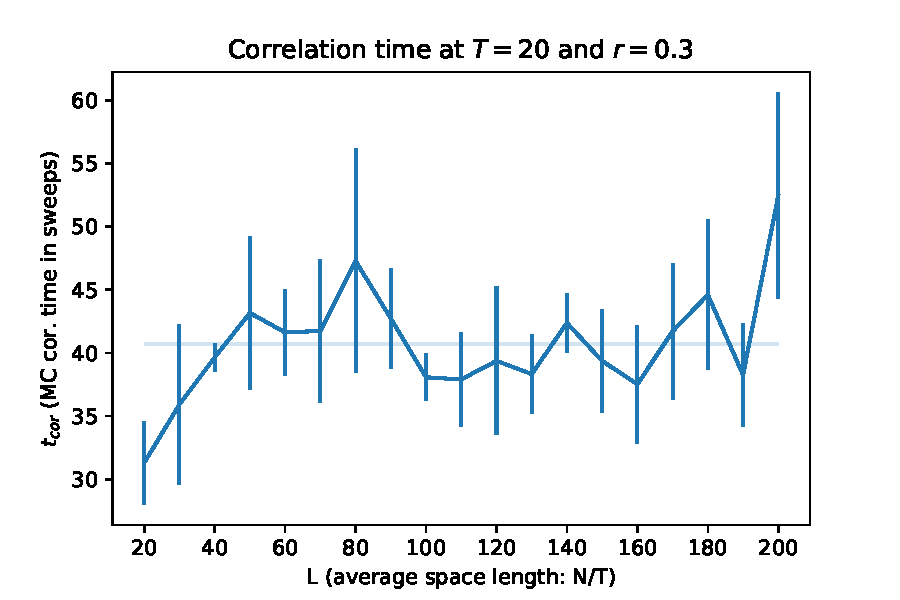
\includegraphics[width=1.0\linewidth]{img/tcor_l_t20_r0.3.pdf}
        \caption{Correlation time at $T = 20$ for different $L$, with corresponding fit.}
        \label{fig:tcor_L}
    \end{minipage}
    \hfill
    \begin{minipage}{0.48\linewidth}
        \centering
        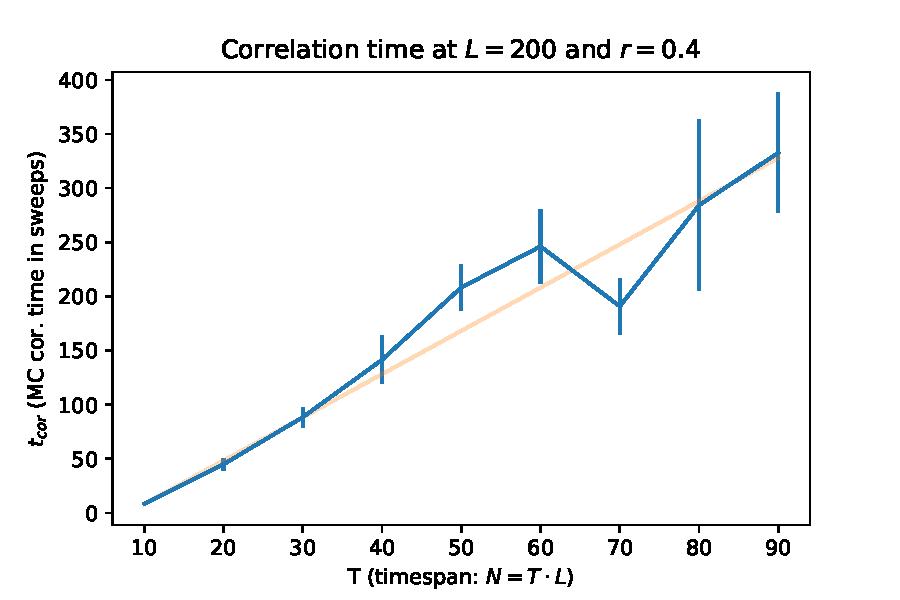
\includegraphics[width=1.0\linewidth]{img/tcor_t_l200_r0.4.pdf}
        \caption{Correlation time at $L = 200$ for different $T$, with corresponding fit.}
        \label{fig:tcor_T}
    \end{minipage}
\end{figure}
From Fig. \ref{fig:tcor_L} it seems that \emph{in terms of sweeps} the correlation time is roughly constant under $L$ and can at $T = 20$ taken to be $t_\text{cor} = 41 \, \text{sweeps}$.
However, under changing $T$ the autocorrelation time seems to be growing roughly linearly, giving the curse approximation $t_\text{cor} \approx 4\, (T - 10)$ that can be use as an estimate for the correlation time for a wanted system size.
This estimate is very crude, but keep in mind that the final results do not actually depend on this measurement of the correlation time. It helps to know the correlation time to be able to only save relevant data, but it will not affect the final results.
So this approximation is sufficient for the purposes of this simulation.

Note that this linear scaling in $T$ of the correlation time (in terms of sweeps), means that the amount of Markov-chain Monte Carlo steps grows like $N^{3/2}$ for a constant ratio $T/L$. This scaling means that our computation time will increase like $N^{3/2}$ the system size is increased, and puts a limit on the system sizes that can be measured.

\paragraph{Discussion} Later in the project we realised that the system sizes of interest were those where $L \ll T$, which is not the case for the systems the equilibration time and correlation time are measured for.
Re-computation of these quantities takes a lot of computational effort, and there was unfortunately not enough time available to do this.
Experience showed that taking $200 \text{sweeps}$ as burn-in time is also sufficient in this regime, and that the correlation time still scales with $N^{3/2}$ for a constant $T/L$ ratio.
The crude approximation for the correlation time does however not seem to be accurate for larger $T/L$ ratio's, as the correlation times seem lower than this estimate would suggest.

%TODO  add to this discussion

\subsection{Measurements}
Now that we have the equilibration and correlation time, we can start to measure observables.
We wish to compare the measured standard deviation and covariance to the theoretical expectation of 2D CDT, which are given in the $T \rightarrow \infty$ limit.
To simulate measurements in this limit we wish to choose $T$ such that $L \ll T$; in this case we use $T = 20 \, L$ as larger values of $T$ have a large impact on computation time.
We can then compute the \emph{length profile} over a range of $L$ values.
Within time constraints, we were able to measure a range of $L = 15, 20, \dots, 50$; we performed $100$ measurements on each at $\sqrt{0.4 \, N}$ intervals, which is chosen as the correlation time appears to be roughly $t_\text{cor} \approx 3 \sqrt{N}$ at this $T/L$ ratio.

\paragraph{Standard deviation}
% Presentation of the results of the standard deviation of the length profile
The data from the simulation can be analysed to obtain estimates for the standard deviation, and by Eq. \eqref{eq:std_ell} estimates for $\Lambda$.
From Eq. \eqref{eq:exp_ell} we expect the cosmological constant and equivalently the standard deviation to depend on the system size like:
\begin{equation}\label{eq:std_theory}
    \Exp{\Lambda} = \frac{1}{L^2}, \qquad \Exp{\sigma_\ell} = \frac{L}{\sqrt{2}} \approx 0.71 \, L.
\end{equation}

To estimate the standard deviation and the error in the estimation from the length profile the standard deviation is determined at every measurement, according to Eq. \eqref{eq:std_meas}, after which \emph{batching} is used.
To make the estimate using batching the measurements are divided into batches -- these must be larger than the correlation time, which for this measurement was the case when dividing in 10 batches -- and the average is taken of every batch.
The averages obtained from the batches can now be treated as identically independently distributed variables -- we then also check there is no significant correlation between the obtained averages.
Then the standard deviation can be estimated by taking the mean of the averages of the batches, and the error in the mean is estimated by taking the standard deviation of the averages of the batches and dividing by $\sqrt{\text{batch count} - 1}$; in other words $\sigma_\ell$ is estimated the standard way by using the batch averages as the independent measurements.

The results of this analysis for the different values of $L$ is presented in Fig. \ref{fig:std_estimate} together with a power-law fit ($a \, e^{\nu}$).
\begin{figure}[ht]
    \begin{minipage}[t]{0.49\linewidth}
        \centering
        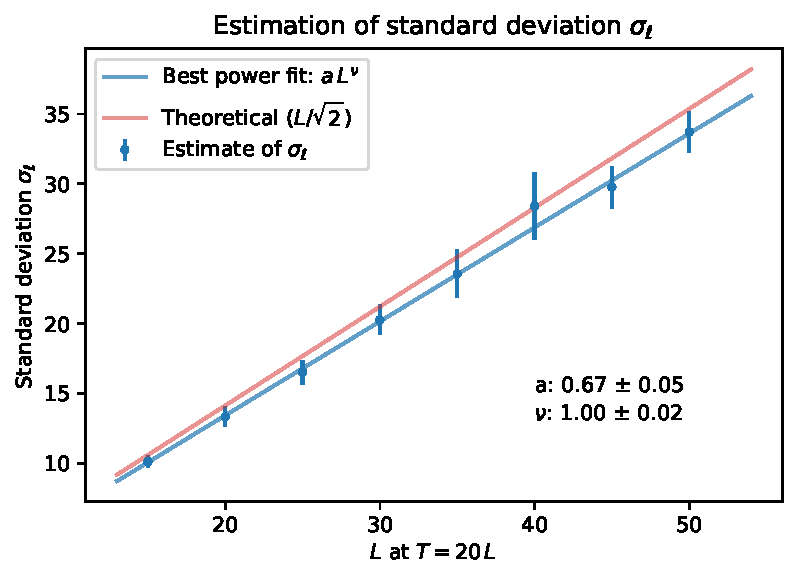
\includegraphics[width=\linewidth]{img/std_estimate.pdf}
        \caption{Measurement results of $\sigma_\ell$ for different system sizes $L$, with power-law fit and theoretical expectation.}
        \label{fig:std_estimate}
    \end{minipage}
    \hfill
    \begin{minipage}[t]{0.49\linewidth}
        \centering
        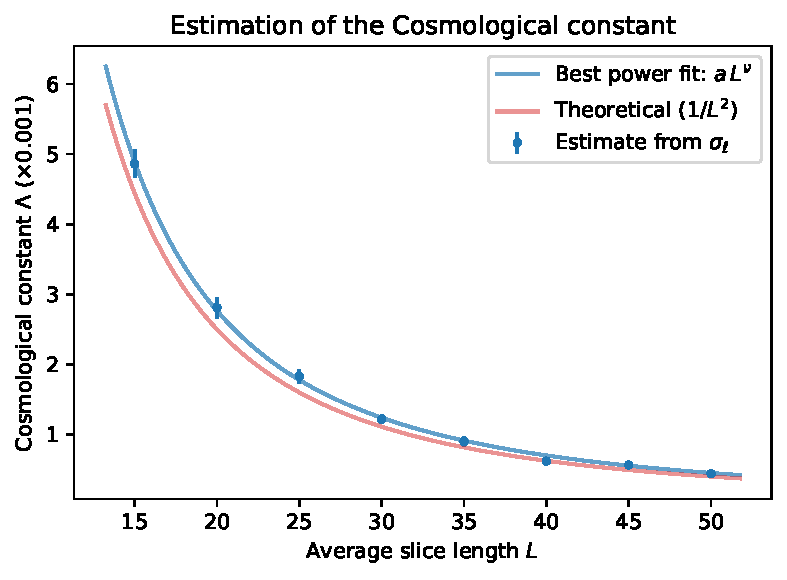
\includegraphics[width=\linewidth]{img/Lambda_estimate.pdf}
        \caption{Estimates for $\Lambda$ based on the $\sigma_\ell$ measurements, with power-law fit and theoretical expectation.}
        \label{fig:Lambda_estimate}
    \end{minipage}
\end{figure}
For the fit is found that $a = 0.67 \pm 0.05$ and $\nu = 1.00 \pm 0.02$, thus we see that as expected by Eq. \eqref{eq:std_theory} $\sigma_\ell$ indeed grows linearly in $L$ with good accuracy and $1/\sqrt{2}$ falls within the $68\%$ confidence interval of $a$. \\
However, from the plot in Fig. \ref{eq:std_ell} it seems that the measurements systematically underestimate the standard deviation.
Since the theoretical result falls within the error, this may simply be coincidence and requires more measurements to decrease the error.
However, this is likely a systematic error made due to having finite $T$, as $\ell(t)$ can only change a finite amount between adjacent timeslices, so having a finite $T$ means that $\ell(t)$ can possibly not fluctuate as far from $L$ as it could for $T \rightarrow \infty$.
To investigate this, and in general the effect of different $T/L$ ratio's, these measurements should be repeated for different values of $T$.
It would be very interesting to get a better view on how the results convergence under increasing $L$, but unfortunately we could not measure this within the time constraint of this project.

From the estimates of $\sigma_\ell$ we can also estimate the cosmological constant $\Lambda$ of the simulated systems, which is used later. This is done simply by the transformation of stochastic variables $\Lambda = 1/2\sigma_\ell^2$, and transforming the mean value and error as usual.
The resulting $\Lambda$ estimates for different $L$ are displayed in Fig. \ref{fig:Lambda_estimate}. From this no real additional information can be extracted as it is simply a transformation, but we can confirm that the cosmological constant closely relates to $L$ with the expected relation \eqref{eq:std_theory}.



\paragraph{Length covariance}
% Presentation of the results of the analysis of the length correlation of the length profile
Next we can also analyse the \emph{length covariance} from the measured length profiles, and compare then to the theoretical covariance \eqref{eq:cov_ell}.
We compute the covariance for every measurement according to Eq. \eqref{eq:cov_meas} and use the same batching method to estimate the covariance and error for every $t$ (again using 10 batches).
The resulting estimates are displayed in Fig. \ref{fig:cov_plot} with $68\%$ confidence intervals.
\begin{figure}[ht]
    \begin{minipage}[t]{0.49\linewidth}
        \centering
        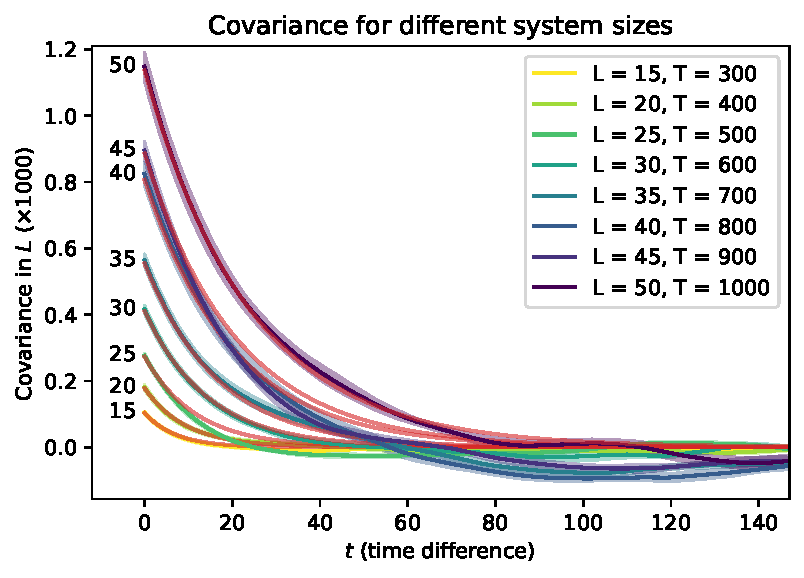
\includegraphics[width=\linewidth]{img/cov_L.pdf}
        \caption{Estimates of the length covariance, labelled by $L$ and show in units of $1000$.}
        \label{fig:cov_plot}
    \end{minipage}
    \hfill
    \begin{minipage}[t]{0.49\linewidth}
        \centering
        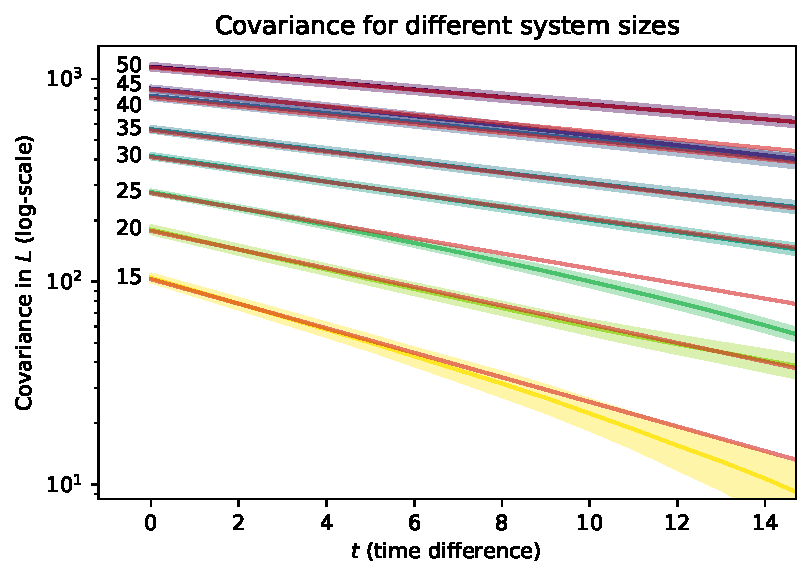
\includegraphics[width=\linewidth]{img/cov_L_log.pdf}
        \caption{Log plot of the length covariance, labelled by $L$ and including theoretical covariance.}
        \label{fig:cov_log_plot}
    \end{minipage}
\end{figure}

Now to compare these measurement results to theory it is important to realise that Eq. \eqref{eq:cov_ell} are only valid for $t \ll T$, which makes it difficult to fit a general exponential through the measured covariance as this exponential relation is only expected to hold for small $t$.
An alternative is to visualise the theoretical covariance alongside the measured covariance such that we can at least visually inspect whether the data matches the expected results.
To plot the theoretical covariance \eqref{eq:cov_ell}, a value for $\Lambda$ is required.
The obvious choice is to let $\Lambda = 1/L^2$ as is theoretically expected.
However, we know from the measurements of $\sigma_\ell$ that it is underestimated, and since $\sigma_\ell^2$ is precisely the normalisation of the covariance using $\Lambda = 1/L^2$ would mean we have this underestimation for all $t$.
And because we already analysed $\sigma_\ell$, the absolute magnitude of the covariance is not that interesting; it is much more interesting to look whether the exponent of the covariance matches theoretical expectations.
For this reason, we use the values of $\Lambda$ estimated for the different $L$ as seen in Fig. \ref{fig:Lambda_estimate}, such that we can check whether the rate of decay relates to the respective estimate of $\Lambda$ in the correct way.
The theoretical covariance with these $\Lambda$ are also plotted in Fig. \ref{fig:cov_plot} in red, but are not very clearly visible.
So to see the relevant behaviour at small $t$ better, Fig. \ref{fig:cov_log_plot} show the same data for small $t$ with a logarithmic $y$-axis.

From Fig. \ref{fig:cov_log_plot} it appears that for small $t$ the measured covariance is indeed linear as expected for the logarithmic plot. And comparing it to the theoretical covariance plotted in red, it seems that the measured covariance also shows the correct exponent, represented by the slope in the logarithmic plot.
For larger $t$ there is deviation from the theoretical line, which it to be expected as the theoretical equation has higher order corrections for larger $t$.

Another way to visualise how well the covariance for different $L$ fit the theoretically expected covariance \eqref{eq:cov_ell} is to scale the covariance and the time difference $t$ such that all covariance measurements should collapse around one curve.
To do this we scale the covariance by $2\Lambda$ and $t$ by $1/2\sqrt{\Lambda}$, such that all curves should collapse around $\exp(-t)$.
The results of scaling are displayed in Fig. \ref{fig:cov_collapsed} as well as a logarithmic plot for small $t$ in Fig. \ref{fig:cov_log_collapsed}, along with $\exp(-t)$ in red.
\begin{figure}[ht]
    \begin{minipage}[t]{0.49\linewidth}
        \centering
        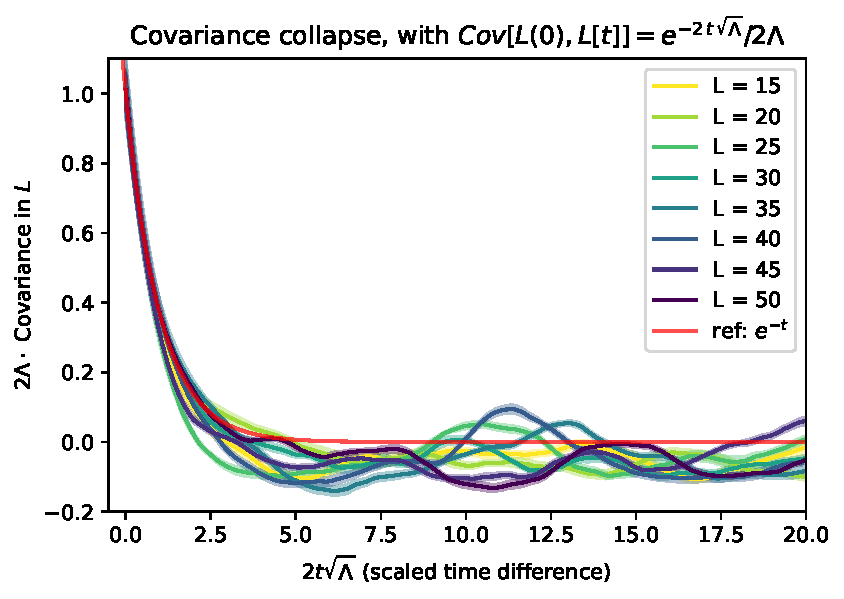
\includegraphics[width=\linewidth]{img/cov_collapsed.pdf}
        \caption{Scaled covariance with reference collapse function in red.}
        \label{fig:cov_collapsed}
    \end{minipage}
    \hfill
    \begin{minipage}[t]{0.49\linewidth}
        \centering
        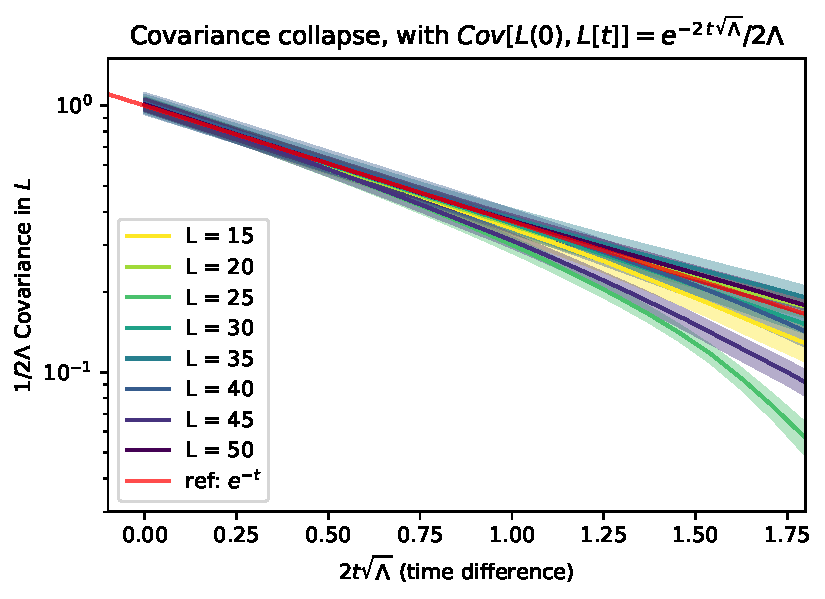
\includegraphics[width=\linewidth]{img/cov_collapsed_log.pdf}
        \caption{Logarithmic plot of scaled covariance.}
        \label{fig:cov_log_collapsed}
    \end{minipage}
\end{figure}
From these plots it is evident that the curves collapse well for small $t$, and that there are discrepancies for larger $t$ as expected.

To make this more quantitative we would want to fit the expected covariance with a general exponential function and compare the different estimation of $\Lambda$ as a result of this fit to each other and to $L$.
However, to be able to fit an exponential we need a large enough part of the covariance $\rho_\ell(t)$ for which $t$ can be considered `small'.
This means that $T$ needs to be larger for a given $L$ than we currently use.
It may also be possible to include higher order terms in the theoretical prediction of the covariance such that the theoretical prediction is valid for larger $t$.
Finally, since what we really want is to find the exponent of Eq. \eqref{eq:cov_ell} for small $t$ and this is equal to the slope at $t = 0$, we might be able to get a reasonable approximation of this slope by considering only the first few points and for example using spline interpolation or a polynomial fit to find the slope at $t=0$.

% \paragraph{Timothy's formula's}
Uit hoofdstuk 4.1 van arXiv:1203.3591 kun je afleiden dat in de continue
limiet met een tijdsinterval T en kosmologische constante $\Lambda$ de
covariantie van de ruimtelijke lengtes $L(t)$ in de limiet $T$ naar oneindig gegeven wordt door
\begin{equation}
    \text{Cov}\big(\ell(0), \ell(t)\big) = \Exp{\qty(\ell(0) - L)\qty(\ell(t) - L)}
    = \frac{1}{2\Lambda} e^{- 2\abs{t}\sqrt{\Lambda}}
\end{equation}
terwijl de verwachtingswaarde gelijk is aan
\begin{equation}
    \Exp{\ell(t)} = \frac{1}{\sqrt{\Lambda}} = L
\end{equation}
In deze limiet van grote $T$ is het de verwachting dat het niet veel
uitmaakt of het totale volume vastgezet wordt of dat er een
kosmologische constante genomen wordt (wat is de juiste relatie tussen
volume en $\Lambda$ in dit geval?).

Kun je deze covariantie zien in de data (tenminste voor $\abs{t} \ll T$)? En is
de constante in de $e$-macht daar ook gerelateerd aan $\Exp{L(t)}$?


\subsection{Discussion}
% Discussion of the interpretation and validity of the results
% Explaination of the difficulties in determining useful results
% Suggestions on improving these measurements
The measurements of the standard deviation $\sigma_\ell$ and of the covariance $\rho_\ell(t)$ agree with the theoretical predictions.
The main concern is the found results have a systematic underestimation of the standard deviation and thus also the covariance as explained due to finite $T$.
So, what should really be done to better understand the dependence of the results on $T$ is to repeat these measurements on different $T/L$ ratio's.
However, since the computation time increases with $N^{3/2}$, this put constraints on system sizes that can be simulated within a reasonable amount of time.

The determination of the equilibration time and correlation time is important to performing the simulation.
However, for this project great effort was taken to determine these times to reasonable accuracy to be able to predict $t_\text{eq}$ and $t_\text{cor}$ for any given $T$ and $L$.
Knowing the computational effort that went into determining these still rather inaccurate predictions, doing it this way is likely not worth it; it is much more fruitful to pick the system sizes one wishes to simulate carefully and determine the equilibration and correlation time for these systems specifically.
Unfortunately, we only later in the project realised what the interesting system sizes were, so we could not optimally use the determined $t_\text{eq}$ and $t_\text{cor}$ anyway.
Also, although we expect $t_\text{eq}$ to be independent of $T$, it should be checked to really make sure any system one does measurements one is thermalised.
If this is not the case and the total amount of measurements is low, the first few measurements could contribute to a significant error to the end results.

Finally, there are many more interesting observable to measure in 2D CDT, some of which are already discussed in section \ref{sec:observables}.
If the time permits it is highly recommended measuring some of these observables, but we could not find the time in this project to look at these.